\begin{center}
	\begin{tabular}{M{9.25cm}M{8.75cm}}
		\textbf{TRƯỜNG THCS-THPT NGUYỄN KHUYẾN}& \textbf{ÔN TẬP KTTX LẦN 2 HỌC KÌ I}\\
		\textbf{MÃ ĐỀ: 001}& \textbf{Bài thi môn: VẬT LÝ 10}\\
		\textit{(Đề thi có 05 trang)}& \textit{Thời gian làm bài: 40 phút, không kể phát đề}
		
		\noindent\rule{4cm}{0.8pt} \\
	\end{tabular}
\end{center}
\setcounter{section}{0}
\section{Câu trắc nghiệm nhiều phương án lựa chọn}
\textit{Thí sinh trả lời từ câu 1 đến câu 20. Mỗi câu hỏi thí sinh chọn một phương án}
\setcounter{ex}{0}
\Opensolutionfile{ans}[ans/D10-HKI-KTTX2-001-TN]
% ===================================================================
\begin{ex}
	Đơn vị đo lực (newton) được viết theo các đơn vị cơ bản trong hệ SI là
	\choice
	{$\si{\kilogram/\meter^2}$}
	{$\si{\kilogram/\second^2}$}
	{$\si{\kilogram\cdot\meter^2/\second}$}
	{\True $\si{\kilogram\cdot\meter/\second^2}$}
	\loigiai{}
\end{ex}
% ===================================================================
\begin{ex}
	Phát biểu nào sau đây là đúng?
	\choice
	{\True Khi vận tốc của vật thay đổi thì chắc chắn đã có lực tác dụng lên vật}
	{Nếu không chịu lực nào tác dụng thì vật phải đứng yên}
	{Khi không chịu lực nào tác dụng lên vật thì vật đang chuyển động sẽ lập tức dừng lại}
	{Vật chuyển động được là nhờ có lực tác dụng lên nó}
	\loigiai{}
\end{ex}
% ===================================================================
\begin{ex}
	Nhận định nào dưới đây về lực là \textbf{chính xác nhất}?\\
	Lực là đại lượng đặc trưng cho tác dụng của vật này lên vật khác. Dưới tác dụng của lực
	\choice
	{vật sẽ chuyển động thẳng đều hoặc quay tròn đều}
	{vật sẽ thu gia tốc và chuyển động biến đổi}
	{vật sẽ bị biến dạng}
	{\True vật sẽ thay đổi trạng thái chuyển động hoặc biến dạng}
	\loigiai{}
\end{ex}

% ===================================================================
\begin{ex}
	Trong chuyển động thẳng chậm dần đều thì hợp lực tác dụng vào vật
	\choice
	{\True ngược chiều chuyển động và có độ lớn không đổi và khác không}
	{cùng chiều chuyển động và có độ lớn giảm dần}
	{ngược chiều chuyển động và có độ lớn giảm dần}
	{cùng chiều chuyển động và có độ lớn không đổi và khác không}
	\loigiai{}
\end{ex}
% ===================================================================
\begin{ex}
	Phát biểu nào sau đây là đúng?
	\choice
	{Vật luôn luôn chuyển động cùng chiều với hợp lực tác dụng lên nó}
	{\True Gia tốc của vật luôn cùng chiều với hợp lực tác dụng lên nó}
	{Hợp lực tác dụng lên vật giảm dần thì vật chuyển động chậm dần}
	{Hợp lực tác dụng lên vật không đổi thì vật chuyển động thẳng đều}
	\loigiai{}
\end{ex}
% ===================================================================
\begin{ex}
	Một vật đang chuyển động với vận tốc $v$. Nếu bỗng nhiên các lực tác dụng lên nó mất đi thì vật
	\choice
	{chuyển động chậm dần rồi dừng lại}
	{đổi hướng chuyển động}
	{\True chuyển động thẳng đều}
	{dừng lại ngay}
	\loigiai{}
\end{ex}
% ===================================================================
\begin{ex}
	Nhìn chiếc xe tải chạy trên đoạn đường thẳng nằm ngang với vận tốc không đổi, ta có thể tin rằng
	\choice
	{người lái xe đã cho động cơ ngừng hoạt động và xe tiếp tục chạy theo quán tính}
	{trên xe không có hàng hóa, ma sát xuất hiện là rất bé và không làm thay đổi vận tốc của xe}
	{\True lực tác dụng của động cơ làm cho xe chuyển động cân bằng với tất cả các lực cản tác dụng lên xe}
	{hợp lực của lực động cơ và mọi lực cản là một lực không đổi và cùng hướng chuyển động của xe}
	\loigiai{}
\end{ex}
% ===================================================================
\begin{ex}
Cho hai lực $\vec{F}_1$ và $\vec{F}_2$ đồng quy. Hai lực phải thỏa điều kiện nào sau đây để độ lớn hợp của hai lực bằng 0?
	\choice
	{Hai lực có độ lớn bằng nhau}
	{Hai lực song song, ngược chiều}
	{\True Hai lực song song, ngược chiều và có độ lớn bằng nhau}
	{Hai lực song song, cùng chiều và có độ lớn bằng nhau}
	\loigiai{}
\end{ex}
% ===================================================================
\begin{ex}
	Một vật đang chuyển động dưới tác dụng của lực không đổi $\vec{F}_1$ với gia tốc $a_1$. Nếu tăng độ lớn lực tác dụng thành $F_2=2F_1$ thì gia tốc của vật là $a_2$. Mối liên hệ giữa $a_2$ và $a_1$ là
	\choice
	{$a_1=2a_2$}
	{$a_2=a_1$}
	{\True $a_2=2a_1$}
	{$a_2=4a_1$}
	\loigiai{}
\end{ex}

% ===================================================================
\begin{ex}
	\immini{Con chó săn to khỏe và chạy nhanh hơn thỏ. Tuy nhiên khi thỏ bị chó săn rượt đuổi, thỏ vẫn có thể thoát nạn nhờ vận dụng chiến thuật luôn luôn đổi hướng chạy đột ngột làm chó săn lỡ đà. Điều này dựa vào tính chất nào trong vật lý?}{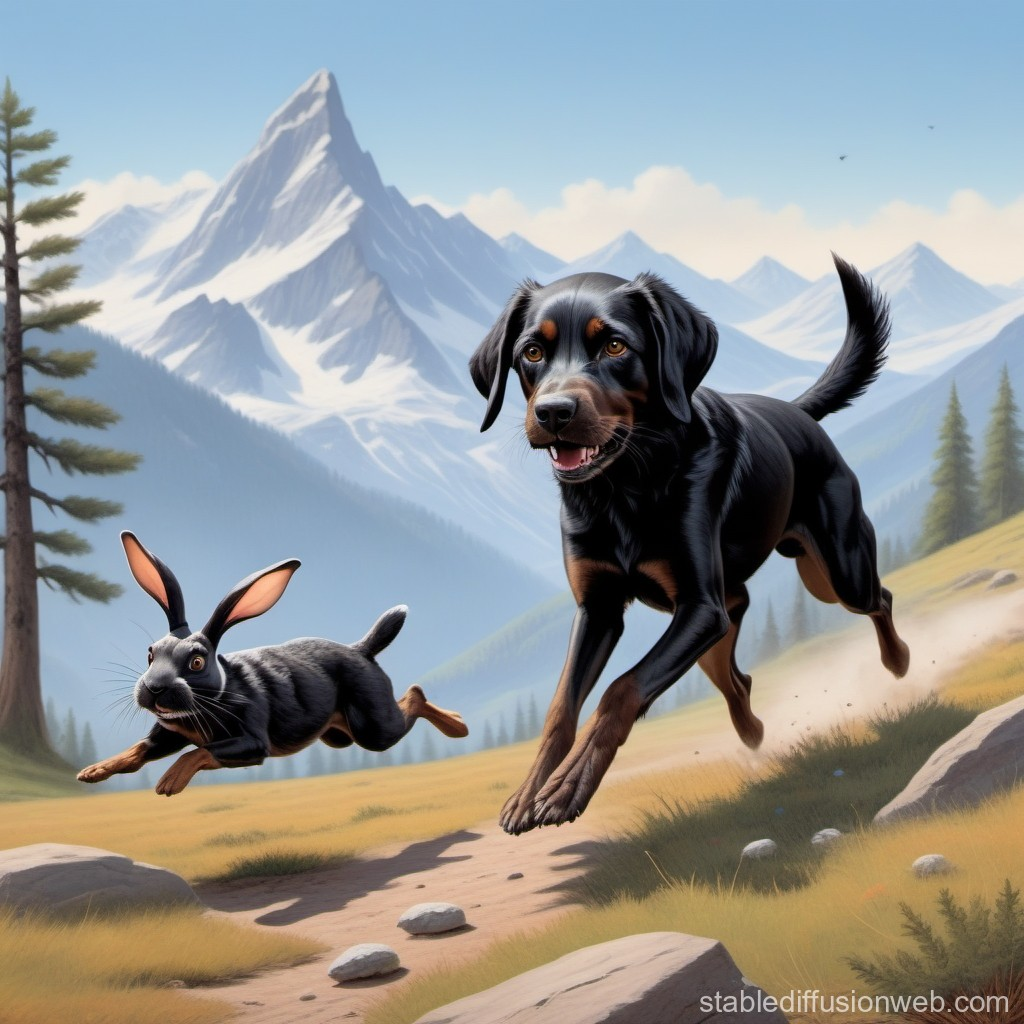
\includegraphics[scale=0.075]{figs/D10-HKI-KTTX2-001-1}}
	\choice
	{Trọng lượng}
	{Lực}
	{\True Quán tính}
	{Vận tốc}
	\loigiai{}
\end{ex}
% ===================================================================
\begin{ex}
Một chất điểm chịu tác dụng của một lực $\vec{F}$ có độ lớn $\SI{20}{\newton}$. Nếu hai lực thành phần của lực đó vuông góc với nhau	và có độ lớn lần lượt là $F_1=\SI{12}{\newton}$ và $F_2$ thì $F_2$ bằng
	\choice
	{\True $\SI{8}{\newton}$}
	{$\SI{16}{\newton}$}
	{$\SI{32}{\newton}$}
	{$\SI{20}{\newton}$}
	\loigiai{}
\end{ex}
% ===================================================================
\begin{ex}
Hai lực khác phương $\vec{F}_1$ và $\vec{F}_2$ có độ lớn $F_1=F_2=\SI{20}{\newton}$, góc tạo bởi hai lực này là $\SI{60}{\degree}$. Hợp lực của hai lực này có độ lớn là	
	\choice
	{$\SI{14.1}{\newton}$}
	{\True $\xsi{20\sqrt{3}}{\newton}$}
	{$\SI{17.3}{\newton}$}
	{$\SI{20}{\newton}$}
	\loigiai{}
\end{ex}
% ===================================================================
\begin{ex}
	Một chất điểm đứng yên dưới tác dụng của 3 lực có giá đồng quy và có độ lớn lần lượt là $\SI{8}{\newton}$, $\SI{10}{\newton}$, $\SI{12}{\newton}$. Nếu bỏ đi lực $\SI{10}{\newton}$ thì hợp lực của hai lực còn lại là
	\choice
	{$\SI{20}{\newton}$}
	{$\SI{6}{\newton}$}
	{$\SI{4}{\newton}$}
	{\True $\SI{10}{\newton}$}
	\loigiai{}
\end{ex}
% ===================================================================
\begin{ex}
	Hai vật có cùng khối lượng bắt đầu chuyển động dưới tác dụng của hai lực cùng phương, cùng chiều và có độ lớn $F_1>F_2$. Quãng đường $s_1$, $s_2$ mà hai vật đi được trong cùng một khoảng thời gian sẽ thỏa
	\choice
	{$\dfrac{s_1}{s_2}=\dfrac{F_2}{F_1}$}
	{\True $\dfrac{s_1}{s_2}=\dfrac{F_1}{F_2}$}
	{$\dfrac{s_1}{s_2}>\dfrac{F_2}{F_1}$}
	{$\dfrac{s_1}{s_2}<\dfrac{F_2}{F_1}$}
	\loigiai{}
\end{ex}
% ===================================================================
\begin{ex}
Sau thời gian $\SI{0.02}{\second}$ tiếp xúc với chân của cầu thủ, quả bóng khối lượng $\SI{500}{\gram}$ ban đầu đứng yên sẽ bay đi với tốc độ $\SI{54}{\kilo\meter/\hour}$. Lực tác dụng lên quả bóng có độ lớn là	
	\choice
	{$\SI{250}{\newton}$}
	{\True $\SI{375}{\newton}$}
	{$\SI{1.35}{\kilo\newton}$}
	{$\SI{13.5}{\kilo\newton}$}
	\loigiai{}
\end{ex}
% ===================================================================
\begin{ex}
	Cho hai lực đồng quy có độ lớn bằng $\SI{8}{\newton}$ và $\SI{12}{\newton}$. Giá trị của hợp lực \textbf{không thể} nhận giá trị nào trong các giá trị sau đây?
	\choice
	{$\SI{7}{\newton}$}
	{$\SI{19}{\newton}$}
	{$\SI{4}{\newton}$}
	{\True $\SI{21}{\newton}$}
	\loigiai{}
\end{ex}
% ===================================================================
\begin{ex}
	Cho hai lực đồng qui có cùng độ lớn $\SI{600}{\newton}$. Nếu hợp lực của hai lực cũng có độ lớn bằng $\SI{600}{\newton}$ thì góc giữa 2 lực bằng
	\choice
	{$\SI{0}{\degree}$}
	{$\SI{180}{\degree}$}
	{$\SI{60}{\degree}$}
	{\True $\SI{120}{\degree}$}
	\loigiai{}
\end{ex}
% ===================================================================
\begin{ex}
	Một chất điểm đứng yên dưới tác dụng của 3 lực có độ lớn bằng nhau. Kết luận nào sau đây là đúng?
	\choice
	{Có 2 lực cùng giá, ngược chiều nhau}
	{Ba lực có giá cùng nằm trong một mặt phẳng, trong đó 2 lực có giá vuông góc nhau}
	{\True Ba lực có giá cùng nằm trong một mặt phẳng và đôi một hợp nhau góc $\SI{120}{\degree}$}
	{Có 2 lực cùng giá, cùng chiều nhau}
	\loigiai{}
\end{ex}
% ===================================================================
\begin{ex}
	Một vật nhỏ có khối lượng $\SI{2}{\kilogram}$, lúc đầu đứng yên. Nó bắt đầu chịu tác dụng đồng thời của hai lực $F_1=\SI{4}{\newton}$ và $F_2=\SI{3}{\newton}$. Góc giữa $\vec{F}_1$ và $\vec{F}_2$ bằng $\SI{30}{\degree}$. Quãng đường vật đi được sau $\SI{1.2}{\second}$ \textbf{gần nhất} với giá trị nào?
	\choice
	{$\SI{2}{\meter}$}
	{\True $\SI{2.45}{\meter}$}
	{$\SI{2.88}{\meter}$}
	{$\SI{3.16}{\meter}$}
	\loigiai{}
\end{ex}
% ===================================================================
\begin{ex}
	Một lực $\vec{F}$ không đổi truyền cho một vật có khối lượng $m_1$ một gia tốc bằng $\SI{4}{\meter/\second^2}$, truyền cho một vật khác có khối lượng $m_2$ một gia tốc bằng $\SI{2}{\meter/\second^2}$. Nếu đem ghép hai vật đó làm một vật thì lực $\vec{F}$ truyền cho vật ghép một gia tốc có độ lớn là
	\choice
	{$\SI{1.03}{\meter/\second^2}$}
	{\True $\SI{1.33}{\meter/\second^2}$}
	{$\SI{3.33}{\meter/\second^2}$}
	{$\SI{3.03}{\meter/\second^2}$}
	\loigiai{}
\end{ex}
\Closesolutionfile{ans}
\section{Câu trắc nghiệm đúng/sai} 
\textit{Thí sinh trả lời từ câu 1 đến câu 2. Trong mỗi ý \textbf{a)}, \textbf{b)}, \textbf{c)}, \textbf{d)} ở mỗi câu, thí sinh chọn đúng hoặc sai}
\setcounter{ex}{0}\\
\Opensolutionfile{ans}[ans/D10-HKI-KTTX2-001-TF]
% ===================================================================
\begin{ex}
	Một bạn học sinh có khối lượng $m=\SI{55}{\kilogram}$ đang thực hiện động tác bật nhảy tại chỗ (jump squat) bằng hai chân trên sàn cứng như hình minh họa bên dưới.
	\immini{
	Tại thời điểm $t_0=0$, học sinh đạt độ cao cực đại và vận tốc bằng 0. Tại thời điểm $t_1$, học sinh này rơi xuống chạm vào mặt sàn bằng hai chân, trọng tâm thân người di chuyển đoạn $h=\SI{0.65}{\meter}$ so với trọng tâm tại thời điểm $t_0$. Để giảm lực tác động lên khớp gối và cột sống trong quá trình tiếp xúc với sàn, bạn này thực hiện động tác gập gối sao cho giữa các thời điểm $t_1$ và $t_2$ trọng tâm của bạn ấy hạ xuống một khoảng $\Delta h=\SI{0.36}{\meter}$.  Trong quá trình rơi trước khi tiếp đất, học sinh rơi nhanh dần đều với gia tốc trọng trường $g=\SI{10}{\meter/\second^2}$ và trọng lực tác dụng lên bạn học sinh được xác định bởi $\vec{P}=m\vec{g}$.
	}
	{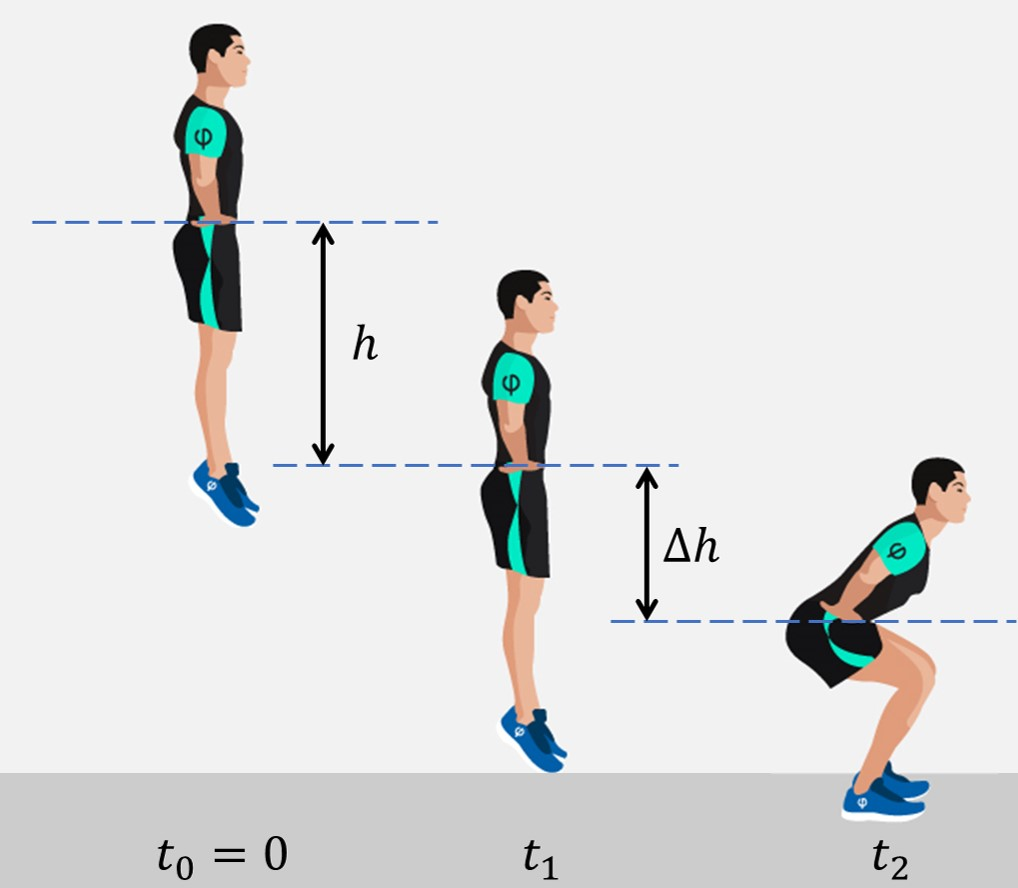
\includegraphics[scale=0.3]{figs/D10-HKI-KTTX2-001-5}}
	\choiceTF[t]
	{\True Tốc độ của bạn học sinh ngay trước khi chạm đất là $\SI{3.6}{\meter/\second}$}
	{\True Gia tốc trung bình của bạn học sinh trong quá trình tiếp đất có độ lớn là $\SI{18}{\meter/\second^2}$}
	{Độ lớn lực cản trung bình do sàn tác dụng lên người trong quá trình tiếp đất là $\SI{990}{\newton}$}
	{\True Thời gian mà bạn học sinh tiếp đất là $\SI{0.2}{\second}$}
	\loigiai{
	\begin{itemchoice}
		\itemch Đúng. $v=\sqrt{2gh}\approx\SI{3.6}{\meter/\second}$.
		\itemch Đúng. $a=\dfrac{-v^2}{2\Delta h}\approx\SI{18}{\meter/\second^2}$.
		\itemch  Sai. $F_c=m\left(g+\left|a\right|\right)\approx\SI{1540}{\newton}$.
		\itemch Đúng. $\Delta t=\dfrac{-v}{a}\approx\SI{0.2}{\second}$.
	\end{itemchoice}
	}
\end{ex}
% ===================================================================
\begin{ex}
	Một người dùng đòn gánh dài $\SI{1.8}{\meter}$ để gánh hai vật $m_1=\SI{20}{\kilogram}$ và $m_2=\SI{25}{\kilogram}$ như hình vẽ. 
	\begin{center}
		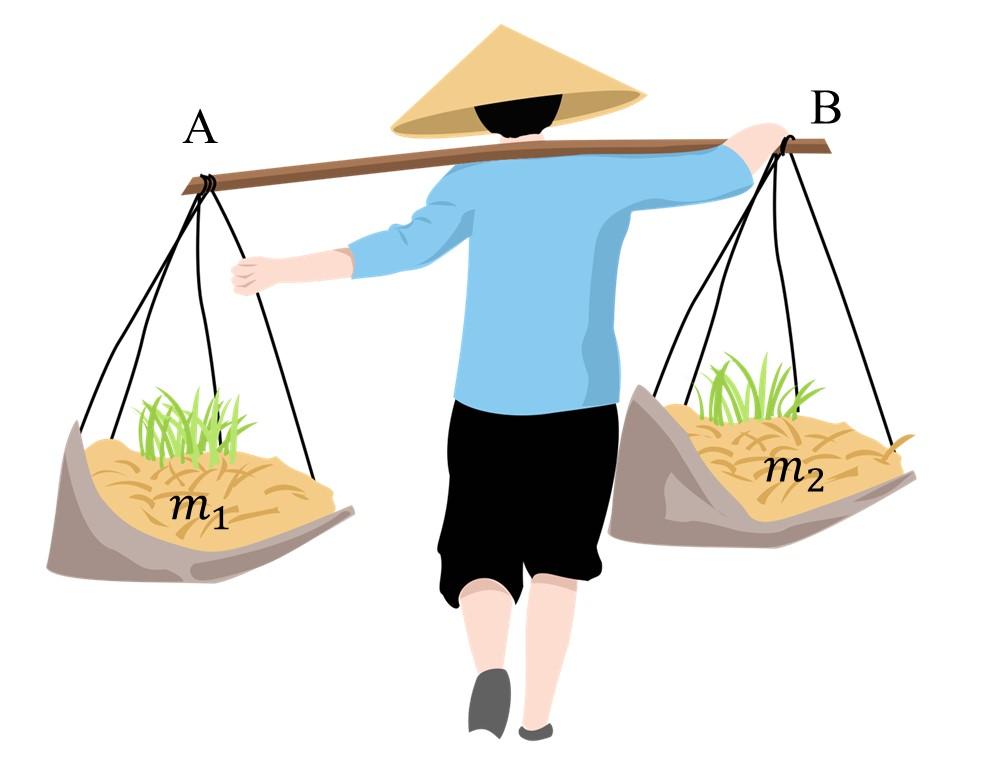
\includegraphics[width=0.3\linewidth]{figs/D10-HKI-KTTX2-001-3}
	\end{center}
	Biết điểm treo hai quang gánh được đặt sát hai đầu đòn gánh, bỏ qua khối lượng của đòn gánh.  Lấy trọng lượng bằng 10 lần khối lượng $P=10m$.
	\choiceTF[t]
	{Trọng lực của vật $m_1$ tác dụng lên đầu A và trọng lực của vật $m_2$ tác dụng lên đầu B là như nhau}
	{\True Điểm đặt vai của người chịu tác dụng của hai lực song song cùng chiều}
	{Để đòn gánh nằm ngang thì vai người đặt ở vị trí chính giữa của đòn gánh}
	{\True Khi gánh nằm ngang thì lực đòn gánh tác dụng lên vai là $\SI{450}{\newton}$ và vai cách đầu A đoạn $\SI{1}{\meter}$}
	\loigiai{
		\begin{itemchoice}
			\itemch Sai. $P_1=\SI{200}{\newton}$; $P_2=\SI{250}{\newton}$.
			\itemch Đúng.
			\itemch Sai. $\dfrac{d_2}{d_1}=\dfrac{P_1}{P_2}=\dfrac{4}{5}$ mà $d_1+d_2=\SI{1.8}{\meter}\Rightarrow \begin{cases}
				d_1=\SI{1}{\meter}\\
				d_2=\SI{0.8}{\meter}
			\end{cases}$.
			\itemch Đúng.
		\end{itemchoice}
	}
\end{ex}
\Closesolutionfile{ans}
\section{Câu trắc nghiệm trả lời ngắn} \textit{Thí sinh trả lời từ câu 1 đến câu 6}
\setcounter{ex}{0}
\Opensolutionfile{ans}[ans/D10-HKI-KTTX2-001-TL]
% ===============================================================
\begin{ex}
	Siêu xe Pininfarina Battista sản xuất tại Italy, được trang bị khả năng động học nâng cao nhờ gói khí động học riêng biệt, có khối lượng khoảng $\SI{2000}{\kilogram}$ đang là siêu xe tăng tốc nhanh nhất thế giới khi chỉ cần 2 giây để tăng tốc từ 0 đến $\SI{28}{\meter/\second}$. Lực để tạo ra gia tốc cho xe trong trường hợp này là bao nhiêu kilo newton $\left(\si{\kilo\newton}\right)$?
	\shortans[oly]{28}
	\loigiai{
		
	}
\end{ex}
% ===============================================================
\begin{ex}
	\immini{Một nha sĩ dùng dây cung niềng răng để chỉnh hình răng khểnh cho một bệnh nhân như hình bên. Lực căng của mỗi dây được điều chỉnh để có độ lớn $\SI{18.0}{\newton}$. Tìm độ lớn của hợp lực do sợi dây tác dụng lên chiếc răng theo đơn vị newton $\left(\si{\newton}\right)$. \textit{(Kết quả làm tròn đến chữ số hàng phần mười)}.}
	{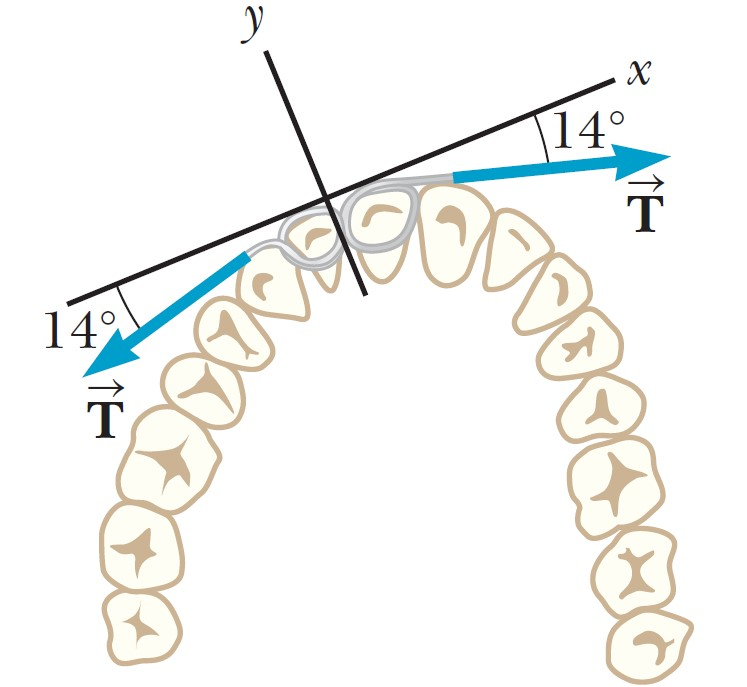
\includegraphics[scale=0.25]{../figs/D10-HKI-KTTX2-002-1}}
	\shortans[oly]{8,7}
	\loigiai{
		
	}
\end{ex}
% ===============================================================
\begin{ex}
	Một ô tô có khối lượng $m=\SI{1000}{\kilogram}$ chuyển động thẳng đều với tốc độ $v=\SI{18}{\kilo\meter/\hour}$ thì tài xế tắt máy xe. Lực ma sát tác dụng lên các bánh xe có độ lớn $\SI{500}{\newton}$ và không đổi. Xe đi thêm được bao xa nữa thì dừng lại?
	\shortans[oly]{25 }
	\loigiai{
		
	}
\end{ex}
% ===============================================================
\begin{ex}
	\immini{Một con nhện đang treo mình dưới một sợi tơ theo phương thẳng đứng thì bị một cơn gió thổi theo phương ngang làm dây treo lệch đi so với phương thẳng đứng một góc $\SI{30}{\degree}$. Biết trọng lượng của con nhện là $P=\SI{0.1}{\newton}$. Xác định độ lớn của lực mà gió tác dụng lên con nhện ở vị trí cân bằng trong hình bên \textit{(làm tròn kết quả đến chữ số hàng phần trăm)}.}
	{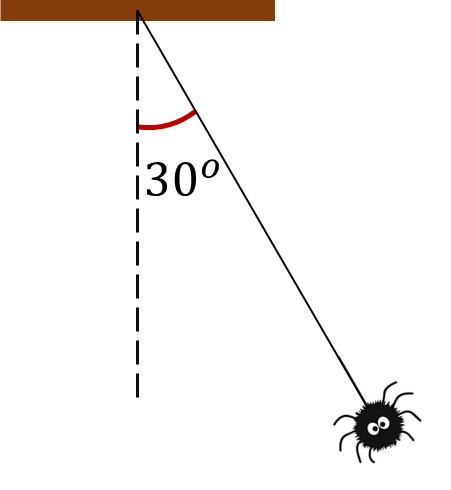
\includegraphics[scale=0.3]{../figs/D10-HKI-KTTX2-001-2}}
	\shortans[oly]{$0,06$}
	\loigiai{
		
	}
\end{ex}
\textit{Dữ kiện dùng chung cho câu 5 và câu 6:}\\
Một vật nhỏ có khối lượng $m=\SI{2}{\kilogram}$ đang nằm yên trên mặt phẳng ngang thì chịu tác dụng của lực kéo $\vec{F}_k$ theo phương nằm ngang. Vật bắt đầu trượt nhanh dần đều với gia tốc $\SI{2}{\meter/\second^2}$. Trong quá trình chuyển động, vật chịu tác dụng của lực cản có độ lớn $\SI{2}{\newton}$.
% ===============================================================
\begin{ex}
Tính độ lớn lực kéo tác dụng lên vật theo đơn vị newton $\left(\si{\newton}\right)$.	
	\shortans[oly]{6}
	\loigiai{
			}
\end{ex}
% ===============================================================
\begin{ex}
Sau khi vật chuyển động được 5 giây, lực kéo ngừng tác dụng. Tính tổng quãng đường vật đi được từ lúc bắt đầu chuyển động đến khi dừng lại theo đơn vị mét $\left(\si{\meter}\right)$.	
	\shortans[oly]{75}
	\loigiai{
		
	}
\end{ex}
\Closesolutionfile{ans}
\begin{center}
	\textbf{--- HẾT ---}
\end{center}